\documentclass[../main.tex]{subfiles}

\begin{document}
\section{Finite difference and Jacobi matrices}

\subsection{Finite differences}
Now we move onto another type of 'infinite matrix' operator, which is used in
practice to discretise differential problems to 'finite difference' problems 
\cite{suli2003introduction}. Much of this section is adapted from \cite{stolz2004seminar}
  and \cite{teschl2000jacobi}.

\begin{definition}[\textbf{Central finite difference and discrete Laplacian}]
  The central finite difference of a function $u: \mathbb{Z} \rightarrow
  \mathbb{C}$ is 
  $$D_c u (n) = \frac{u(n+1) - u(n-1)}{2}.$$
  We can then define the second finite difference, or discrete Laplacian, as
  $\Delta_c = D_c^2$.
\end{definition}

A natural representation of the function $u: \mathbb{Z} \rightarrow \mathbb{C}$
is as a doubly infinite column vector, $$u = (\hdots u(-1), u(0), u(1),\hdots)^T.$$
Then we can represent our finite differences as matrix multiplication of $u$
by a doubly infinite matrix, such as
  $$ 
  D_c = 
  \begin{pmatrix*}[c]
    \ddots & \ddots & & & \\
    \ddots & 0 & 1 & & \\
    & -1 & 0 & 1 & \\
    & & -1 & 0 & \ddots \\
    & & & \ddots & \ddots \\
  \end{pmatrix*}
  \quad\quad
  \Delta_c = 
  \begin{pmatrix*}[c] 
    \ddots & \ddots & & & \\
    \ddots & -2 & 1 & & \\
    & 1 & -2 & 1 & \\
    & & 1 & -2 & \ddots \\
    & & & \ddots & \ddots \\
  \end{pmatrix*}. 
  $$
These infinite tridiagonal matrices are known as Jacobi matrices. The discrete
Laplacian is often transformed into the `free Jacobi matrix' $J_0 = \Delta_c +
2I$, as this simplifies the structure without affecting the spectrum (it only
shifts it over by 2). Another example of a Jacobi matrix is the diagonal
operator $\diag(q)$ for some $q: \mathbb{Z} \rightarrow \mathbb{C}$, defined as
the multiplication operator $\diag(q)v(n) = q(n)v(n)$.
  $$ 
  \diag(u) = 
  \begin{pmatrix*}[c]
    \ddots & \ddots & & & \\
    \ddots & q_{-1} & 0 & & \\
    & 0 & q_0 & 0 & \\
    & & 0 & q_1 & \ddots \\
    & & & \ddots & \ddots \\
  \end{pmatrix*}.
  $$

\begin{remark}
  While discrete and continuous operators may share names, it is important to
  understand that they are not necessarily equivalent, even as approximations:
  for example, we have seen above that the continuous Laplacian has spectrum
  $[0, \infty)$ on $L^2(\mathbb{R})$. On the other hand, the discrete Laplacian
  is a Toeplitz matrix, equivalent to the Toeplitz operator with symbol 
  $e^{i \theta} + e^{-i \theta} - 2$ (intuitively, $\Delta_c = S + S^* - 2I$ with S as the
  shift operator, and multiplying a Fourier series by $e^{i \theta}$
  'shifts all the coefficients along by 1') \cite{arveson2002short}.
  Then by Theorem \ref{thm:hartman-wintner}
  (Hartman-Wintner), it follows that the spectrum of the discrete Laplacian is
  $[-4, 0]$ (using that $e^{i \theta} + e^{-i \theta} = 2cos(\theta)$).
  However, we will shortly see in Example \ref{ex:finite-differences} a method
  of approximating differential operators by Jacobi matrices.
\end{remark}

Note that using the matrix without our original definition (given in general
below) to fall back on raises some issues that must be addressed: if the matrix
is doubly infinite, it doesn't make sense as just an array of values without
taking care to define where the `main diagonal' even is \cite{lindner2013where}!

The above remark showed that the finite difference matrices were Toeplitz, and the
theory of section \ref{sec:toeplitz} applies to them. However, the diagonal
operator is not generally Toeplitz, and the Jacobi matrix begins to be interesting where
it ceases to be generally Toeplitz:

\begin{definition}[\textbf{General second-order finite difference operator}]
\index{finite difference operator}\index{Jacobi operator}\index{Jacobi matrix}
  For any set X, let $X^\mathbb{Z}$ be the set of doubly infinite sequences $\mathbb{Z}
  \rightarrow X$. Consider three sequences:
  $b \in \mathbb{C}^\mathbb{Z}$
  and $a, c \in (\mathbb{C} \setminus 0)^\mathbb{Z}$.\\
  A general second-order finite difference operator 
  $J: \mathbb{C}^\mathbb{Z} \rightarrow \mathbb{C}^\mathbb{Z}$
  is then defined by the action 
  \begin{equation}
  \label{eqn:2efde}
    Ju (n) = a_n u(n-1) + b_n u(n) + c_{n+1} u(n+1).
  \end{equation}
  We will define specific Jacobi operators via the notation $J = J(a, b, c)$
  for convenience.
\end{definition}

As one would expect, this is represented as the Jacobi matrix
  $$ 
  J = 
  \begin{pmatrix*}[c]
    \ddots & \ddots & & & \\
    \ddots & b_{-1} & c_0 & & \\
    & a_0 & b_0 & c_1 & \\
    & & a_1 & b_1 & \ddots \\
    & & & \ddots & \ddots \\
  \end{pmatrix*}.
  $$
Of course, we could similarly define a singly infinite matrix of sequences defined on $\mathbb{N}$
or $\mathbb{N}_0$.

\begin{example}
\label{ex:finite-differences}
  A popular way to solve ODE problems numerically is via \emph{finite difference approximation},
  which is to approximate a differential operator with a singly-infinite Jacobi operator. For
  example, we may want to approximate the Schr\"odinger operator $Hu = -\frac{d^2}{dx^2}u + qu$
  on the half-line $L^2[0, \infty)$, with boundary condition $u \cos(\alpha) + u' \sin(\alpha) = 0$
  as the finite difference operator
  $J(-h^{-2}, \tilde{q}, -h^{-2})$
  where $\tilde{q}$ is defined:
  $$
  \tilde{q} =
  \begin{cases}
    \tilde{q}(0) = \frac{1}{2h^2 * \tan(\alpha)} + \frac{q(x*h)}{2} + 1 \\
    \tilde{q}(k) = \frac{2}{h^2} + q(k*h) & \text{for all other $k$}
  \end{cases}
  $$
  where $h$ is a given constant 'step size', i.e. we approximate the continuous
  potential $q$ on a grid with spacing of $h$ between the points. The boundary
  condition is included in $\tilde{q}(0)$.
\end{example}

\begin{proposition}\label{thm:2efde-sols} 
  Given a Jacobi operator $J$, the initial value problem for some initial points
  $n_0, n_0 + 1$
  $$
  \begin{cases}
    Ju = f\\
    u(n_0) = a\\ u(n_0 + 1) = b
  \end{cases} 
  $$
  has a unique solution.
\end{proposition}
\begin{proof}
We can rearrange equation (\ref{eqn:2efde}) to see that $u(n-1)$ is uniquely
determined by $u(n)$ and $u(n+1)$, and $u_{n+1}$ by $u(n)$ and
$u(n-1)$. This creates a three-term recurrence relation in both directions -
thus an entire sequence $u \in \mathbb{C}^\mathbb{Z}$ can be determined from the two
initial conditions.
\end{proof}

\begin{proposition}
\label{thm:2efde-ker-dim}
  The kernel of $J$, $N_0(J) \eqdef \{u \in \mathbb{C}^\mathbb{Z} : Ju = 0\}$
  is a two-dimensional subspace of $\mathbb{C}^\mathbb{Z}$;
  therefore, the eigenspace of $J$, 
$$N_\lambda(J) \eqdef \{u \in \mathbb{C}^\mathbb{Z} : (J - \lambda)u = 0\}$$
for any eigenvalue $\lambda$, is also two-dimensional.
\end{proposition}
\begin{proof}
For some Jacobi matrix $J$, define a `solution map' 
$S: \mathbb{C}^2 \rightarrow \mathbb{C}^\mathbb{Z}$ which maps pairs of
complex numbers $(a, b)$ to the solution $u$ of 
  $$
  \begin{cases} 
    Ju = 0\\
    u(0) = a\\ u(1) = b.
  \end{cases}
  $$
We now show that $S$ is a linear
isomorphism from $\mathbb{C}^2$ to the kernel $N_0 (J)$.
\begin{enumerate}[I.]
\item First we show $S$ is linear. Consider $a, b, c, d, e \in
\mathbb{C}$, and let $S(a, b) = u$, $S(d, e) = v$. Then by the
linearity of $J$, for $w = cu + v$, $Jw = cJu + Jv = 0$. Then
$w$ solves
  $$ 
  \begin{cases}
    Jw = 0\\
    w(0) = ca + d\\
    w(1) = cb + e 
  \end{cases}
  $$
which by uniqueness must mean $S(c(a, b) + (d, e)) = w = cS(a, b) + S(d, e)$.

\item The injectivity of $S$ is almost immediate: let $S(a, b) = S(c, d) = u$.
Then $u(0) = a$ and $u(0) = c$, therefore $a = c$, and likewise $u(1) = b = d$.

\item Finally, we show that $S$ is surjective. Consider $u \in N_0 (J)$, so $Ju
= 0$, and thus it is clear that $u = S(u(0), u(1)).$ \end{enumerate} Then $S$ is
a linear isomorphism, so we have $\mathbb{C}^2 \cong N_0 (J)$, and so
$\dim(\mathbb{C}^2) = \dim(N_0 (J)) = 2$.

The similar result for eigenspaces follows as
$N_\lambda (J) = N_0 (J - \lambda)$. If $J$ is a Jacobi matrix, so is $J - \lambda$;
it is $J$ but with the sequence $(b_n)_{n \in \mathbb{Z}}$ replaced by $(b_n - \lambda)_{n \in
\mathbb{Z}}$. 
\end{proof}

\subsection{Floquet theory}
For differential operators with a periodic element
(such as Sturm-Liouville operators with periodic potential), their spectral
theory is interwoven with Floquet theory, which can simplify the system down to
the study of a `fundamental matrix'. A similar theory can be developed for
discrete `finite difference' problems - this theory will allow us to
\emph{exactly} solve certain problems with a modification of the truncation
method.

We call a Jacobi matrix $N$-periodic if the sequences $a_n, b_n, c_n$ are all
$N$-periodic.

Consider an operator $M$, which we shall call the \emph{monodromy
operator}\index{monodromy operator}, which intuitively inscribes `what has
happened after one period': $Mu(n) = u(n+N)$. If $u(n)$ is a solution for $Ju =
\lambda u$, then so is $v(n) = u(n+N)$; thus we can consider $M(\lambda)$ as an
operator on $N_\lambda (J)$. Then by Proposition \ref{thm:2efde-ker-dim},
$M(\lambda)$ is an operator on a two-dimensional space, so can be represented as
a $2 \times 2$ matrix with respect to some basis. For simplicity, we can use
$S$, the `solution map' from Proposition \ref{thm:2efde-ker-dim}; as linear
isomorphisms carry a basis to a basis, the two solutions $u_1 = S(1, 0)$ and
$u_2 = S(0, 1)$ are a basis of $N_\lambda (J)$. In this basis we have
  $$
  M(\lambda) =
  \begin{pmatrix}
    u_1(N) & u_2(N) \\
    u_1(N+1) & u_2(N+1)
  \end{pmatrix}
  $$
In the Floquet theory literature, the eigenvalues and eigenvectors of
$M(\lambda)$ are referred to as Floquet multipliers and Floquet solutions
respectively. $M(\lambda)$ must have at least one eigenvalue $z$ for any
$\lambda$, and here is where Floquet theory gets its strength: a Floquet
solution $u$ satisfies $Ju = \lambda u$ and also has the additional property
that $u(n+N) = zu(n).$

In fact, we can obtain (see e.g. \cite{teschl2000jacobi}) that the eigenvalues
of $M(\lambda)$ satisfy the property $z_1 z_2 = 1$, and thus are reciprocal to
each other, i.e. are $z(\lambda), \frac{1}{z(\lambda)}$. We can also use
Floquet solutions in the following \emph{exact} method of calculating
the spectrum for a periodic Jacobi operator.

\begin{theorem}[\textbf{Floquet-Bloch decomposition}]
\index{Floquet-Bloch decomposition} 
  \label{thm:floquet-bloch}
  Let $J$ be the Jacobi operator $J(a_n, b_n, c_n)$. 
  Consider the finite eigenvalue problem $J_z u = \lambda u$, where
  \begin{equation}
  \label{eqn:floquet-bloch}
    J_z =
    \begin{pmatrix*}[c]
      b_1 & c_2 & & & a_1/z(\lambda)\\
      a_2 & b_2 & c_3 & & & \\
      & a_3 & b_3 & \ddots & & \\
      & & \ddots & \ddots & c_N & \\
      c_{N+1} z(\lambda) & & & a_N & b_N\\
    \end{pmatrix*}.
  \end{equation}
Then if $|z|=1$, any eigenvalue $\lambda$ of $J_z$
is in the essential spectrum of $J$.
\end{theorem}

The 'essential spectrum' will be discussed in more detail shortly, in section \ref{sec:ess-spec}.
For now, it suffices to say that the essential spectrum $\Spec_e(T)$ is a subset of the spectrum
characterised as the set of all $\lambda$ such that there is a 'Weyl singular sequence'
$x_n$ satisfying $\|x_n\| = 1$, $(x_n, \phi) \rightarrow 0$ for all $\phi$ in $\hilbert$
(weak convergence), and $\|Tx_n - \lambda x_n\| \rightarrow 0$.

\begin{proof} For the infinite problem, we have that $\tilde{u}$ satisfies
  the eigenvalue equation for $J$ if
  $$a_n \tilde{u}(n-1) + b_n \tilde{u}(n) + c_{n+1} \tilde{u}(n+1) = \lambda \tilde{u}(n)$$
so in particular as $u(n + N) = z u(n)$, 
\begin{align*}
  & \frac{a_1}{z} u(N) + b_1 u(1) + c_2 u(2) = \lambda u(1)\\
  \Rightarrow \quad& a_1 \tilde{u}(0) + b_1 \tilde{u}(1) + c_2 \tilde{u}(2) 
	    = \lambda u(1), \text{ and } \\
  & a_N u(N-1) + b_N u(N) + c_{N+1} z u(1) = \lambda u(N)\\
  \Rightarrow \quad& a_N \tilde{u}(N-1) + b_N \tilde{u}(N) + c_{N+1} \tilde{u}(N+1) 
            = \lambda u(N)
\end{align*}
which is exactly the first and last column of (\ref{eqn:floquet-bloch}). For any values of
$n$ greater than $N$, say $N + k$ for $k \leq N$ 
\begin{align*}
  a_{N+k} \tilde{u}(N+k-1) + b_{N+k} \tilde{u}(N+k) + c_{N+k+1} \tilde{u}(N+k+1)
    & = \lambda u(N+k) \\
  \Rightarrow \quad z a_{k} u(k-1) + z b_{k} u(k) + z c_{k+1} u(k+1) & = \lambda z u(k)
\end{align*} 
where the $z$'s then cancel. $a_{N+k} = a_{k}$ and likewise for $b$ and $c$ due to periodicity.
A similar argument for values less than 1 will give similar results; for $k \geq N$, repeated
application of the procedure will again give the same results for some exponent of $z$.
Thus a solution to our finite problem (\ref{eqn:floquet-bloch}) extends to an `almost-eigenvector'
$\tilde{u}$ (note that $\tilde{u}$ is generally not in $\ell^2$ as it is periodic).

We can now construct the Weyl singular sequence indexed by $k$:
$$
  v_n^{(k)} = {\tilde{u}_n} \rho_n^{(k)}, \text{ where }
  \rho_n^{(k)} =
  \begin{cases}
    \frac{1}{\sqrt{k+1}} & \text{if } |k-n| < k/2 \\
    0 & \text{otherwise.}
  \end{cases}
$$
  The term $\sqrt{k+1}$ is a normalising factor such that $\|v^{(k)}\|_{\ell^2} = 1$.

We first show that $v^{(k)}$ weakly converges to 0. We can use Lemma
\ref{thm:weak-conv-dense-subset} to restrict to showing it for a dense subset
$c_{00}$ of sequences with finite support (that is, sequences which are
all zero for $n \notin [m, M]$, $m, M \in \mathbb{Z}$).

Then we have
\begin{align*}
  (v^{k}, \phi) & =  \sum_{n \in \mathbb{Z}}
  \overline{\tilde{u}_n} \rho_n^{(k)} \phi_n & \\
  & = \sum_{n \in [m, M]} \overline{\tilde{u}_n} \rho_n^{(k)} \Phi 
    & \text{\emph{where $\Phi = \max_{n}(\phi)$}} \\
  & \rightarrow 0 & 
\end{align*}
  as the support of $\rho_n^{(k)}$ is $[k/2, 3k/2]$, which will travel to the 
  right and become disjoint with the support of $\phi$ as $k \rightarrow \infty$.

Finally, we show that $\|Jv^{(k)} - \lambda v^{(k)}\|_{\ell^2} \rightarrow 0$:
\begin{align*}
    \|Jv^{(k)} - \lambda v^{(k)}\|_{\ell^2} & \leq \|Jv^{(k)}\|_{\ell^2}  - \|\lambda v^{(k)}\|_{\ell^2}  \\
    & = \sum_{n \in \mathbb{Z}}|J\tilde{u}_n \rho_n^{(k)}|^2 + \sum_{n \in \mathbb{Z}}|\lambda\tilde{u}_n \rho_n^{(k)}|^2 \\
    & = \sum_{n \in [k/2, 3k/2]}|\frac{J\tilde{u}_n}{\sqrt{1+k}}|^2 + \sum_{n \in [k/2, 3k/2]}|\frac{\lambda\tilde{u}_n}{\sqrt{1+k}}|^2
\end{align*}
  where the summands are zero if $n \neq {1, N}\mod N+1$ (using that $|z| = 1$ to ensure the norm is periodic).
  If $n = 1$, we have error
\begin{align*}
  (\frac{1}{\sqrt{1+k}}|a_1 \tilde{u}_0 + b_1 \tilde{u}_1 + c_2 \tilde{u}_2|^2 - |\frac{a_1}{z}\tilde{u}_N + b_1 \tilde{u}_1 + c_2 \tilde{u}_2|)^2 \\
  \leq (\frac{1}{\sqrt{1+k}}|a_1 \tilde{u}_0|^2 - |a_1 \tilde{u}_N|)^2
\end{align*}
  and if $n = N$,
\begin{align*}
  (\frac{1}{\sqrt{1+k}}|a_N \tilde{u}_N-1 + b_N \tilde{u}_N + c_{N+1} \tilde{u}_N+1|^2 - |c_{N+1}z\tilde{u}_1 + a_N tilde{u}_N-1 + b_N \tilde{u}_N|)^2 \\
  \leq (\frac{1}{\sqrt{1+k}}|c_{N+1} \tilde{u}_{N+1}|^2 - |c_{N+1} \tilde{u}_1|)^2
\end{align*}
This error is always of the order $O(\sqrt{1 + k}) \rightarrow 0$.

Thus $\lambda$ is in $\Spec_e(J)$. \end{proof} From this we have the inclusion
$$\bigcup_{|z|=1} \Spec(J_z) \subseteq \Spec_e(J)$$.

We can, in fact, find equality in this case \cite{teschl2000jacobi}. 
This decomposition is much more
computationally tractable; if we calculate the spectrum of these finite
matrices for some sample of values on the unit circle, we can thus find the
entire spectrum with no pollution. Furthermore, if the period is sufficiently
small, we may well be able to compute the spectrum with a far smaller matrix
than what we would use for the Ritz spectrum.

\begin{example}
\index{almost Mathieu operator} 
The \emph{almost Mathieu operator} on $\ell^2(\mathbb{Z})$, arising in quantum physics,
is famous for being the subject of the `Ten Martini Problem' \footnote{so-called
for the prize offered by Mark Kac - who conjectured a stronger form known as the
`Dry Ten Martini Problem' - for its solution \cite{simon1982almost}.
The conjecture, solved by Avila and Jitomirskaya in 2006 \cite{avila2006ten},
is that if $\alpha$ is irrational, then $\Spec(H_\omega^{\lambda, \alpha})$
is homeomorphic to the Cantor set (a pathological subset of $[0, 1]$ which is 
compact and uncountably large, but is nowhere dense, totally disconnected, and has measure 0).}.
It has the action
  $$H_\omega^{\lambda, \alpha} u(n) = u(n+1) + u(n-1) + 2\lambda \cos(2\pi (\omega + n \alpha))u(n)$$
for $\alpha, \omega \in [0, 2\pi]$ and $\lambda > 0$. As we can see, this
operator is a second-order finite difference operator. Furthermore, if
$\alpha$ is rational, say $\alpha = x/y$, then it is a periodic discrete
Schr\"odinger operator with period $y$.
Let $b_n = 2\lambda \cos(2\pi (\omega + n \alpha))u(n)$, then
\begin{align*} 
  b_{y+n} = 2\lambda \cos(2\pi (\omega + (y + n) \alpha)) 
	& = 2\lambda \cos(2\pi (\omega +  \frac{xy}{y} + n \frac{x}{y})) \\
  & = 2\lambda \cos(2\pi (\omega + x + n \frac{x}{y})) \\
  & = 2\lambda \cos(2\pi (\omega + n \frac{x}{y})) = b_n 
\end{align*}
  as $x$ is an integer and $\cos(2\pi(\cdot))$ is 1-periodic. Thus we can compute the
spectrum exactly via the Floquet-Bloch decomposition. Letting $\alpha$ vary, we can obtain
the famous 'Hofstadter butterfly' \cite{hofstadter1976energy} in Figure \ref{fig:hofstadter-butterfly}.
Note that we know for rational $\alpha$, the operator has purely essential spectrum
by Theorem \ref{thm:floquet-bloch}; as a result,
we know that the additional eigenvalues in the Ritz approximation are polluting. 

\begin{figure}[p!] \centering
\begin{subfigure}{0.9\textwidth}
  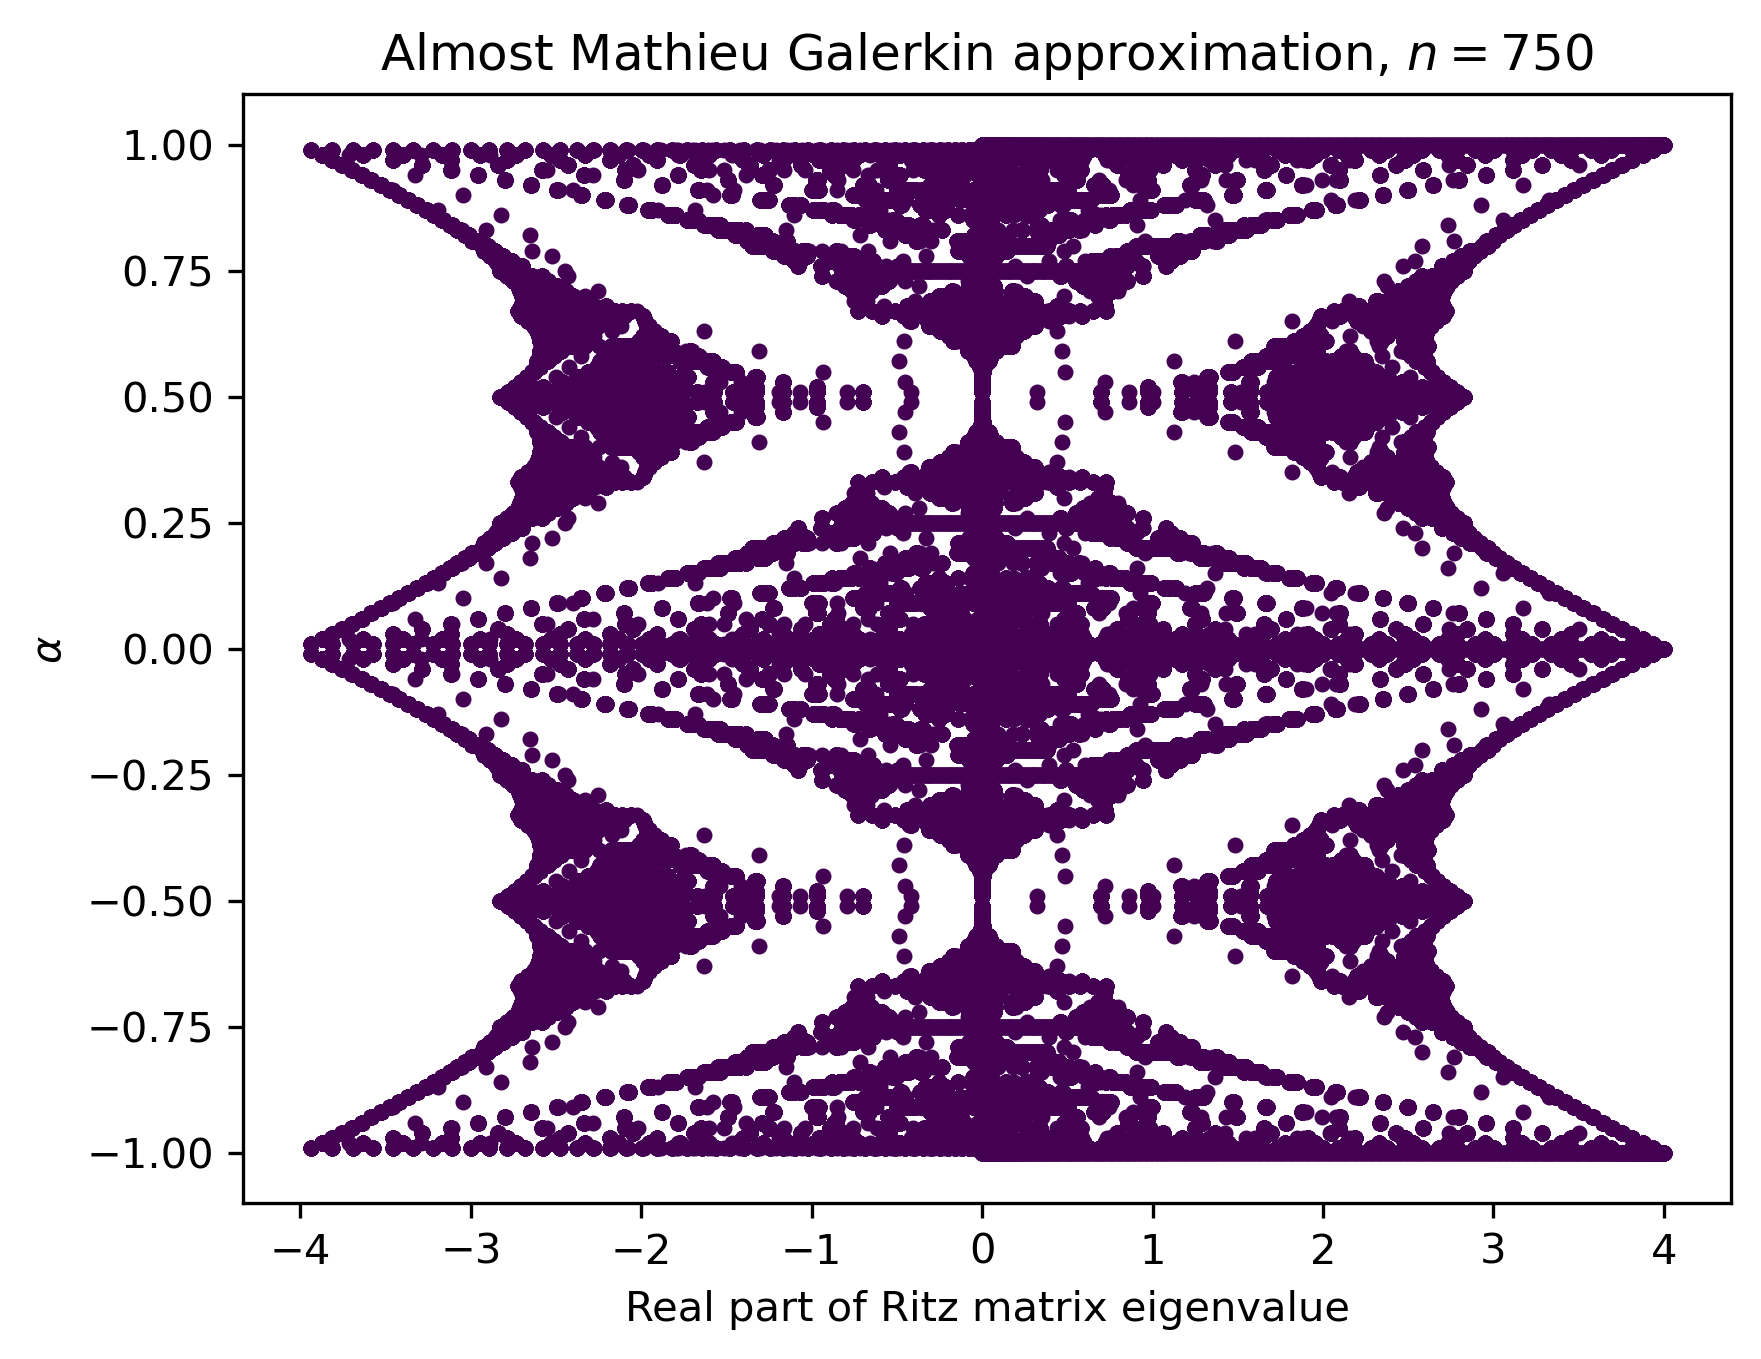
\includegraphics[width=\textwidth]{ten-martini-ritz}
  \end{subfigure}\\
  \begin{subfigure}{0.9\textwidth}
  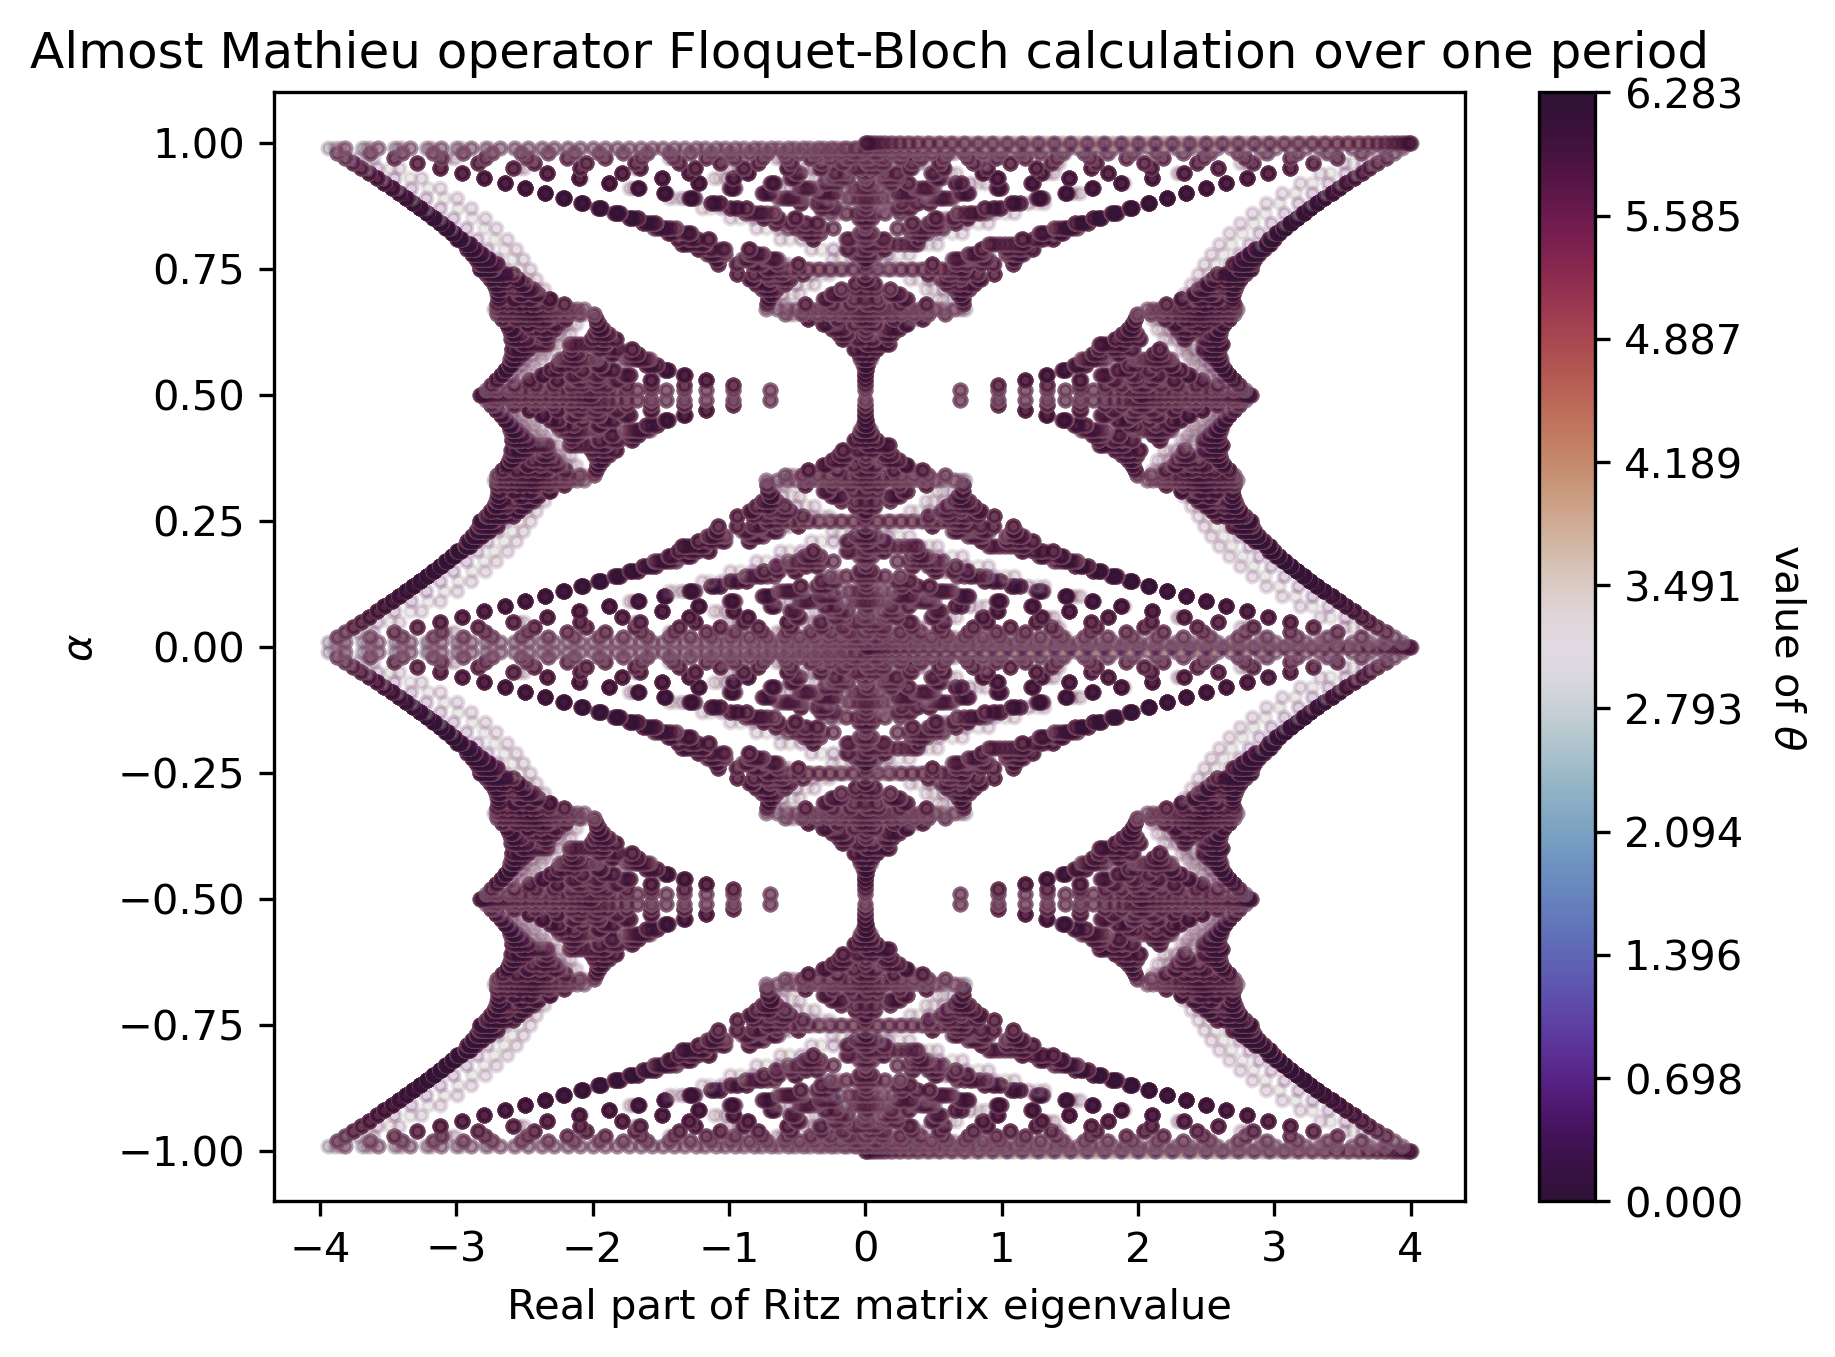
\includegraphics[width=\textwidth]{ten-martini-floquet} \end{subfigure}
\caption{Galerkin and Floquet-Bloch calculation for the almost Mathieu operator, 
  with Floquet-Bloch matrix
	size of one period, and Ritz matrix size of 750.
  Colour is used on the supercell graph to
	distinguish different values of $\theta$, which were 50 evenly
	distributed values between $0$ and $2 \pi$.}

\label{fig:hofstadter-butterfly}
\end{figure}
\clearpage
\end{example}

\subsection{Supercell methods}\index{supercell method} For discrete systems with
a random element, we can adapt the Floquet-Bloch decomposition
via an approach first devised for studying defects in materials with crystal structure
\cite{nieminen2007supercell}. We will discuss these via a physically motivated
example called the \textbf{Feinberg-Zee random hopping model},
\index{Feinberg-Zee model} in the process giving an intuitive explanation
of how the Floquet-Bloch matrix encapsulates periodic behaviour.

These methods are often used heuristically by physicists and crystallographers
and have only been made rigorous in certain cases (e.g. Soussi
\cite{soussi2006convergence} for Heimholtz operators where the potential is
almost periodic with a compactly supported perturbation); for such a simple
idea, the proof is incredibly involved. 

Feinberg and Zee (1999) \cite{feinberg1999nonhermitian} models an unusual
behaviour in superconductors via a class of non-self-adjoint and random
operators on $\ell^2(\mathbb{Z})$: matrices of the form
  $$ 
  A \eqdef
  \begin{pmatrix*}[c]
    \ddots & \ddots & & & & \\
    \ddots & 0 & 1 & & & \\
    & c_{n-1} & 0 & 1 & & \\
    & & c_{n} & 0 & 1 & \\
    & & & c_{n+1} & 0 & \ddots \\
    & & & & \ddots & \ddots & \\ \end{pmatrix*}
  $$
which is the Jacobi operator $J(c_n, 0, 1)$. $c_n$ is a random sequence, where
for a fixed value $\sigma \in (0, 1]$, $c_n$ takes values from $\{-\sigma,
\sigma\}$ at random, taking value $\sigma$ with probability $p$. For random
matrices, it is naturally difficult to discern the entire spectrum (one will
often instead derive an `almost sure' spectrum of what will be in the spectrum
for almost any $p$) \cite{chandler-wilde2012spectrum}.\\

Note that for a discrete problem, the orthonormal basis of $\ell^2(\mathbb{Z})$
are the column vectors $\phi_n = (\delta_{in})_{i \in \mathbb{Z}}$. As a result,
all the Galerkin method is really doing is truncating a doubly infinite matrix
to a finite matrix. Now if we consider an eigenvector $u$ to the truncated
problem, how does it correspond to the original operator? If we denote the
sequence in our truncation as $(c_1, \hdots, c_{n-1})$, then on the infinite
matrix, the operator maps the first entry $u_1$ to $c_0 u_0 + u_2$ and the last
entry $u_{n-1}$ to $c_{n-2} u_{n-2} + u_{n}$. On the other hand, in our
truncation, $u_1$ is mapped to $u_2$, and $u_{n-1}$ to $c_{n-2} u_{n-2}$. In a
way, we have artificially imposed a boundary condition on $u$, in this case
imposing a Dirichlet boundary that $c_k = 0$ for $k \in \mathbb{Z} \setminus
\{1, \hdots, n-1\}$. Is this a valid assumption? Some authors suggest that in
certain cases, spectral pollution may be entirely due to a heavy-handed choice
of imposed boundary \cite{cances2011periodic}.

The supercell method approximates a random tridiagonal matrix by a periodic one.
For our Feinberg-Zee matrix, simply replace the random sequence $c_n$ by a
$k$-periodic sequence $n \mapsto c_{((n \bmod k )+ 1)}$.\footnote{One can see
how this works for sequences on the (super)diagonal similarly. Note there is no
particular relevance to the $+1$; it merely helps bookkeeping by keeping our
indexing from $1$ to $k$.}

  $$ 
  A \eqdef
  \begin{pmatrix*}[c]
    \ddots & \ddots & & & & \\
    \ddots & 0 & 1 & & & \\
    & c_{n-1} & 0 & 1 & & \\
    & & c_{n} & 0 & 1 & \\
    & & & c_{n+1} & 0 & \ddots \\
    & & & & \ddots & \ddots & \\
  \end{pmatrix*}
  \leadsto 
  A^{per} \eqdef
  \begin{pmatrix*}[c]
    \ddots & \ddots & \ddots & & & &\\
    & c_{k-1} & 0 & 1 & & & &\\
    & & c_{k} & 0 & 1 & & &\\
    & & & c_1 & 0 & 1 & \\
    & & &  & c_2 & 0 & \ddots \\
    & & & & & \ddots & \ddots & \\ \end{pmatrix*} $$

We now assume (with some loss of generality that we will later recover) that our
eigenvector $u \in \ell^2(\mathbb{Z})$ is also $k$-periodic. Then if we truncate
the matrix to one period with periodic boundary conditions, then essentially all
of the information of our infinite matrix is retained in the finite case. In
crystallographic terms, we are determining the behaviour of the system from
zooming in on a `unit cell'.

\begin{equation}
\label{eqn:periodising}
  A^{per} \eqdef
  \begin{pmatrix*}[c]
    \ddots & \ddots & \ddots & & & & \\
    & c_{k-1} & 0 & 1 & & & & \\
    & & c_{k} & 0 & 1 & & & \\
    & & & c_1 & 0 & 1 & \\
    & & &  & c_2 & 0 & \ddots \\
    & & & & & \ddots & \ddots & \\
  \end{pmatrix*}
  \leadsto 
  A^{per}_k \eqdef
  \begin{pmatrix*}[c]
    c_1 & 0 & 1 & & & c_{k}\\
    & c_2 & 0 & 1 & & & \\
    & & c_3 & 0 & \ddots & & \\
    & & & \ddots & \ddots & 1 & \\
    1 & & & & c_{k-1} & 0\\ 
  \end{pmatrix*}
\end{equation}

As mentioned previously, on the infinite matrix, the operator maps the first
entry $u_1$ to $c_0 u_0 + u_2$ and the last entry $u_{n-1}$ to $u_{n-2} + c_{n}
u_{n}$. Then in periodic boundary conditions, $u_1$ maps to $c_k u_k + u_2$, and
$u_{k}$ to $c_{k-1} u_{k-1} + u_{1}$, which we represent in matrix form in
equation (\ref{eqn:periodising}) by adding two `corners' to our truncated
tridiagonal matrix. This appears to be a good situation numerically, as we
require almost no extra effort to (apparently) lose far less information.\\

Returning to our generality (where $u$ is not generally $k$-periodic) brings us back to the
Floquet-Bloch decomposition of the operator. If we have the following matrices
$A^{per}_{k, \theta}$ for $\theta \in (0, 2 \pi]$:
  $$ 
  A^{per}_{k, \theta} \eqdef
  \begin{pmatrix*}[c]
    c_1 & 0 & 1 & & & c_{k} e^{i \theta}\\
    & c_2 & 0 & 1 & & & \\
    & & c_3 & 0 & \ddots & & \\
    & & & \ddots & \ddots & 1 & \\
    e^{- i \theta} & & & & c_{k-1} & 0 \\
  \end{pmatrix*} 
  $$
then the Floquet-Bloch decomposition states 
  $$\Spec(A^{per}) = \bigcup_{\theta \in (0, 2 \pi]} \Spec(A^{per}_{k, \theta}).$$
In practice, we take a finite sample of values between 0 and $2 \pi$ for our
$\theta$, and calculate the eigenvalues in each case. 

In Figure \ref{fig:feinberg-zee} one can see a comparison between the Galerkin
and supercell approximations for the Feinberg-Zee model. 

\begin{figure}[h!]
\centering
\begin{subfigure}{0.9\textwidth}
  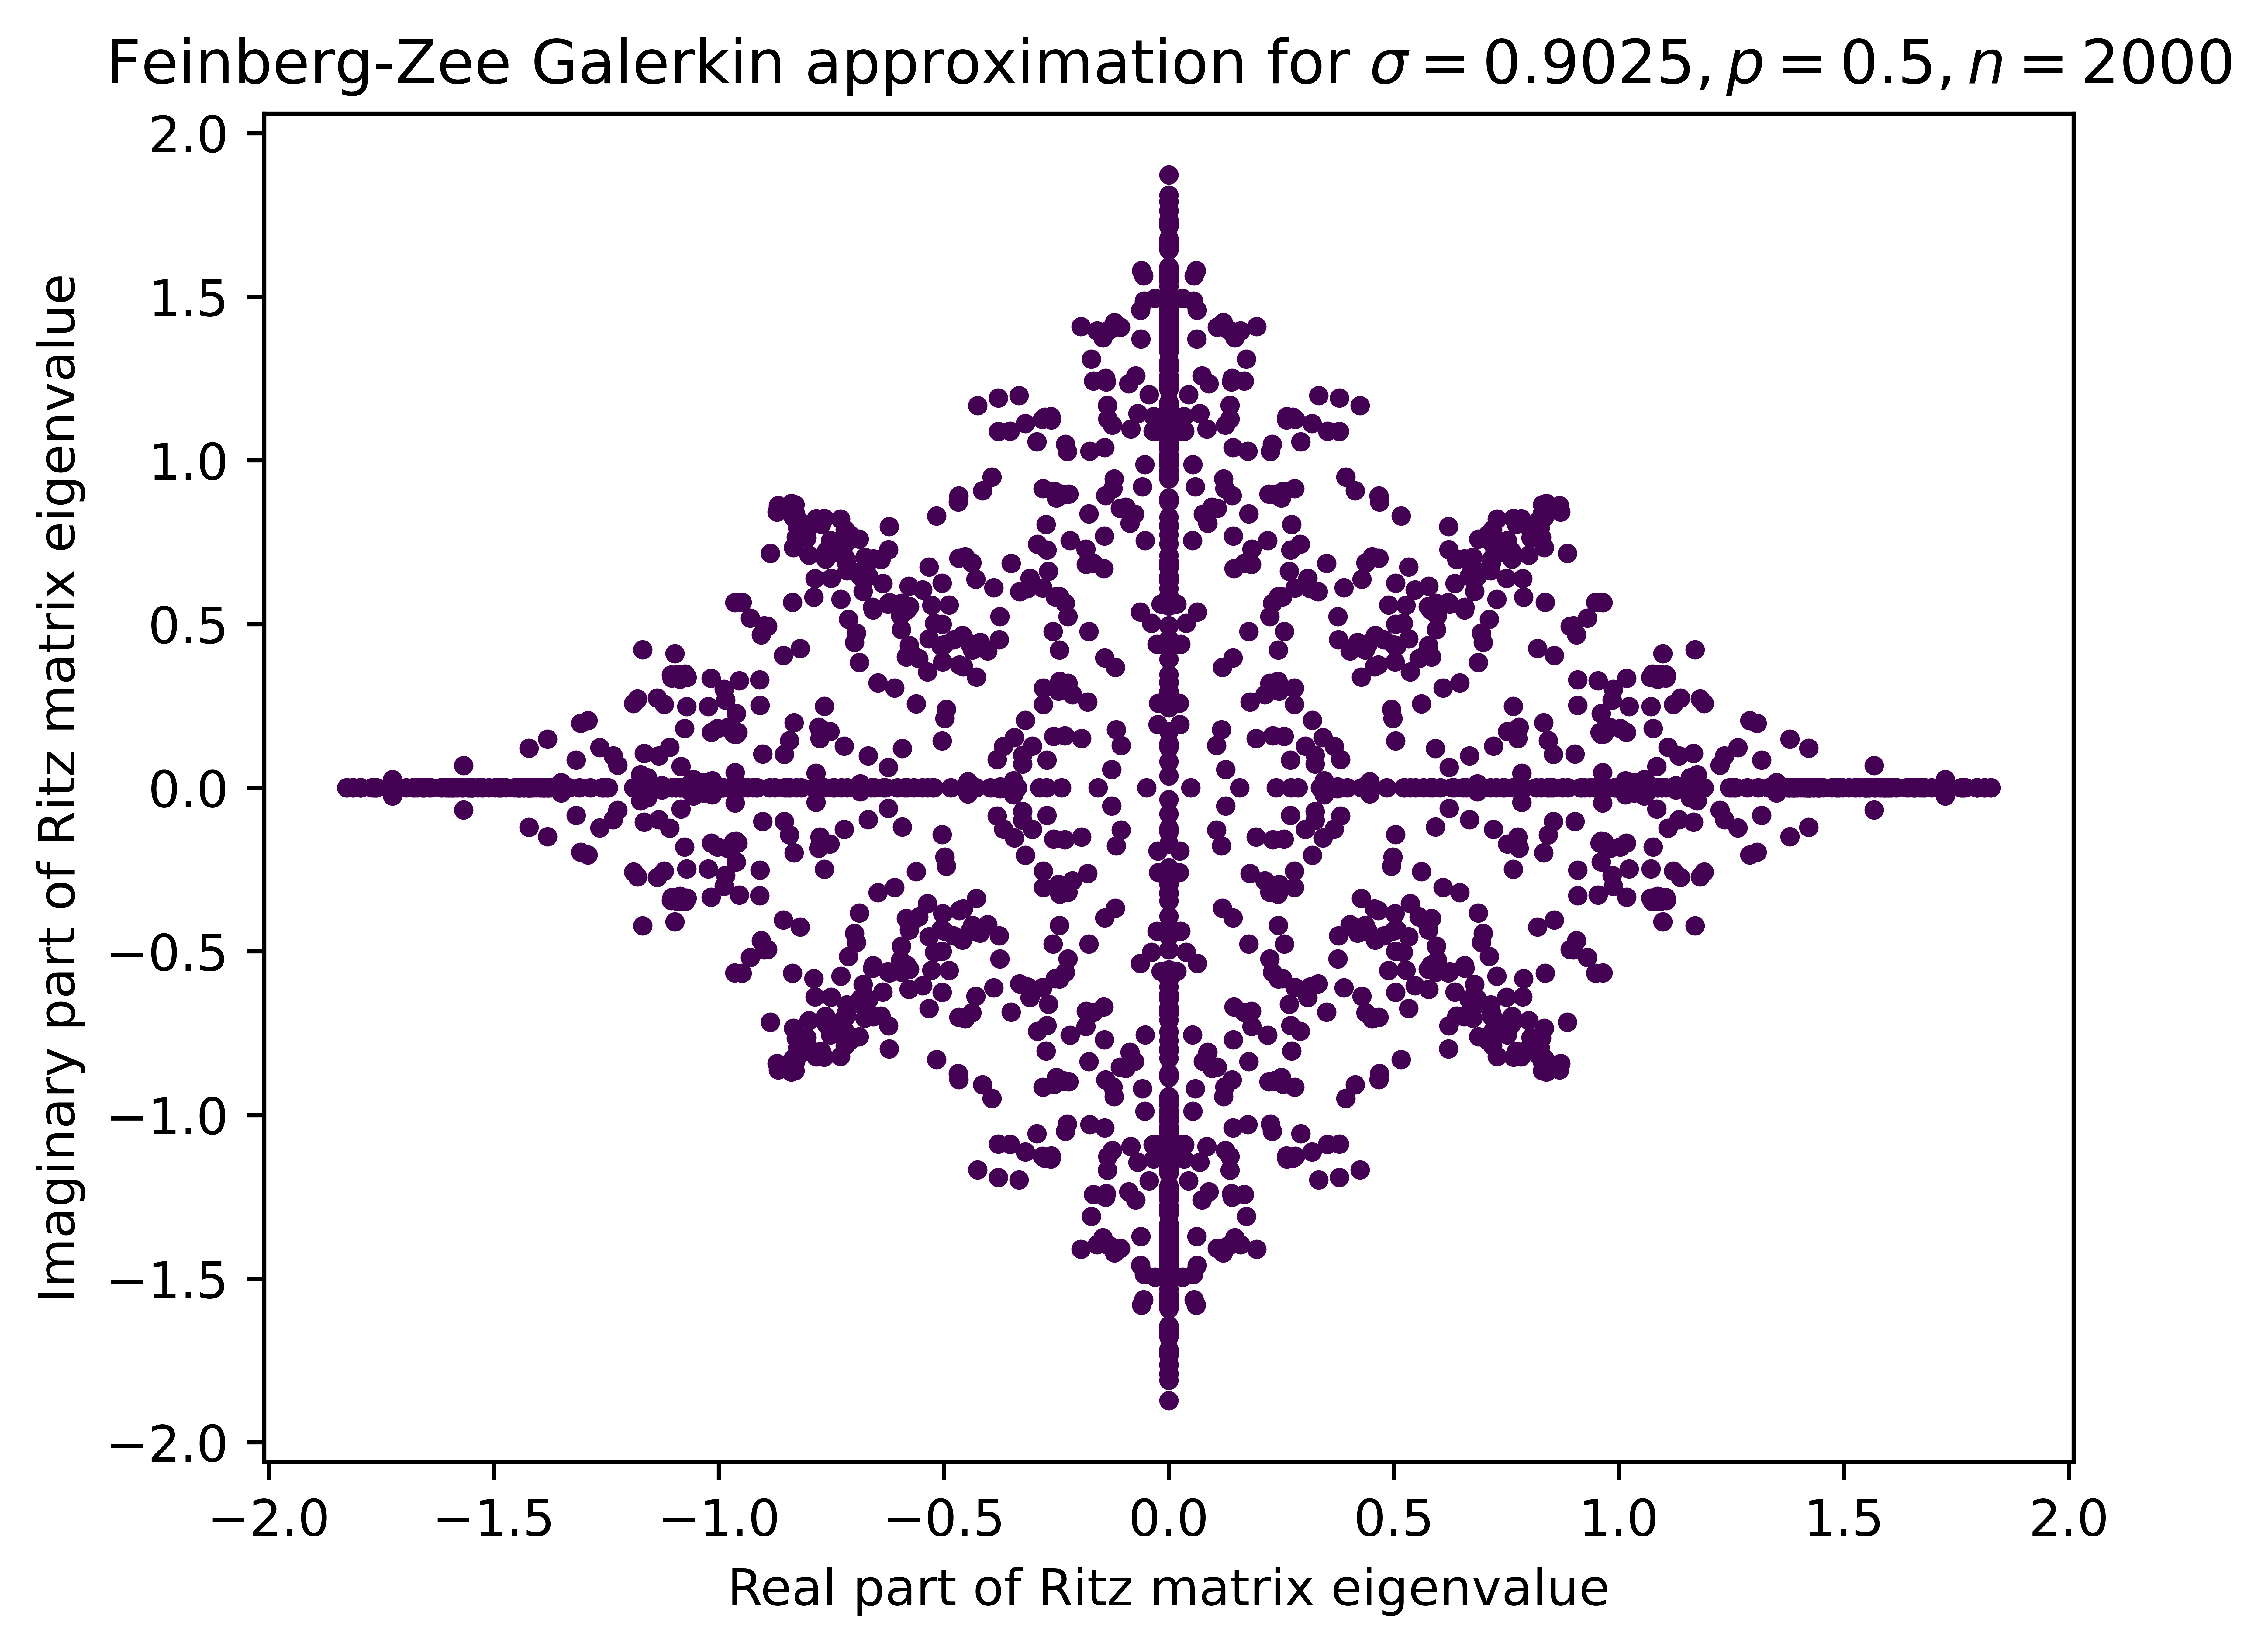
\includegraphics[width=\textwidth]{feinberg-zee-galerkin}
  \end{subfigure}\\
  \begin{subfigure}{0.9\textwidth}
  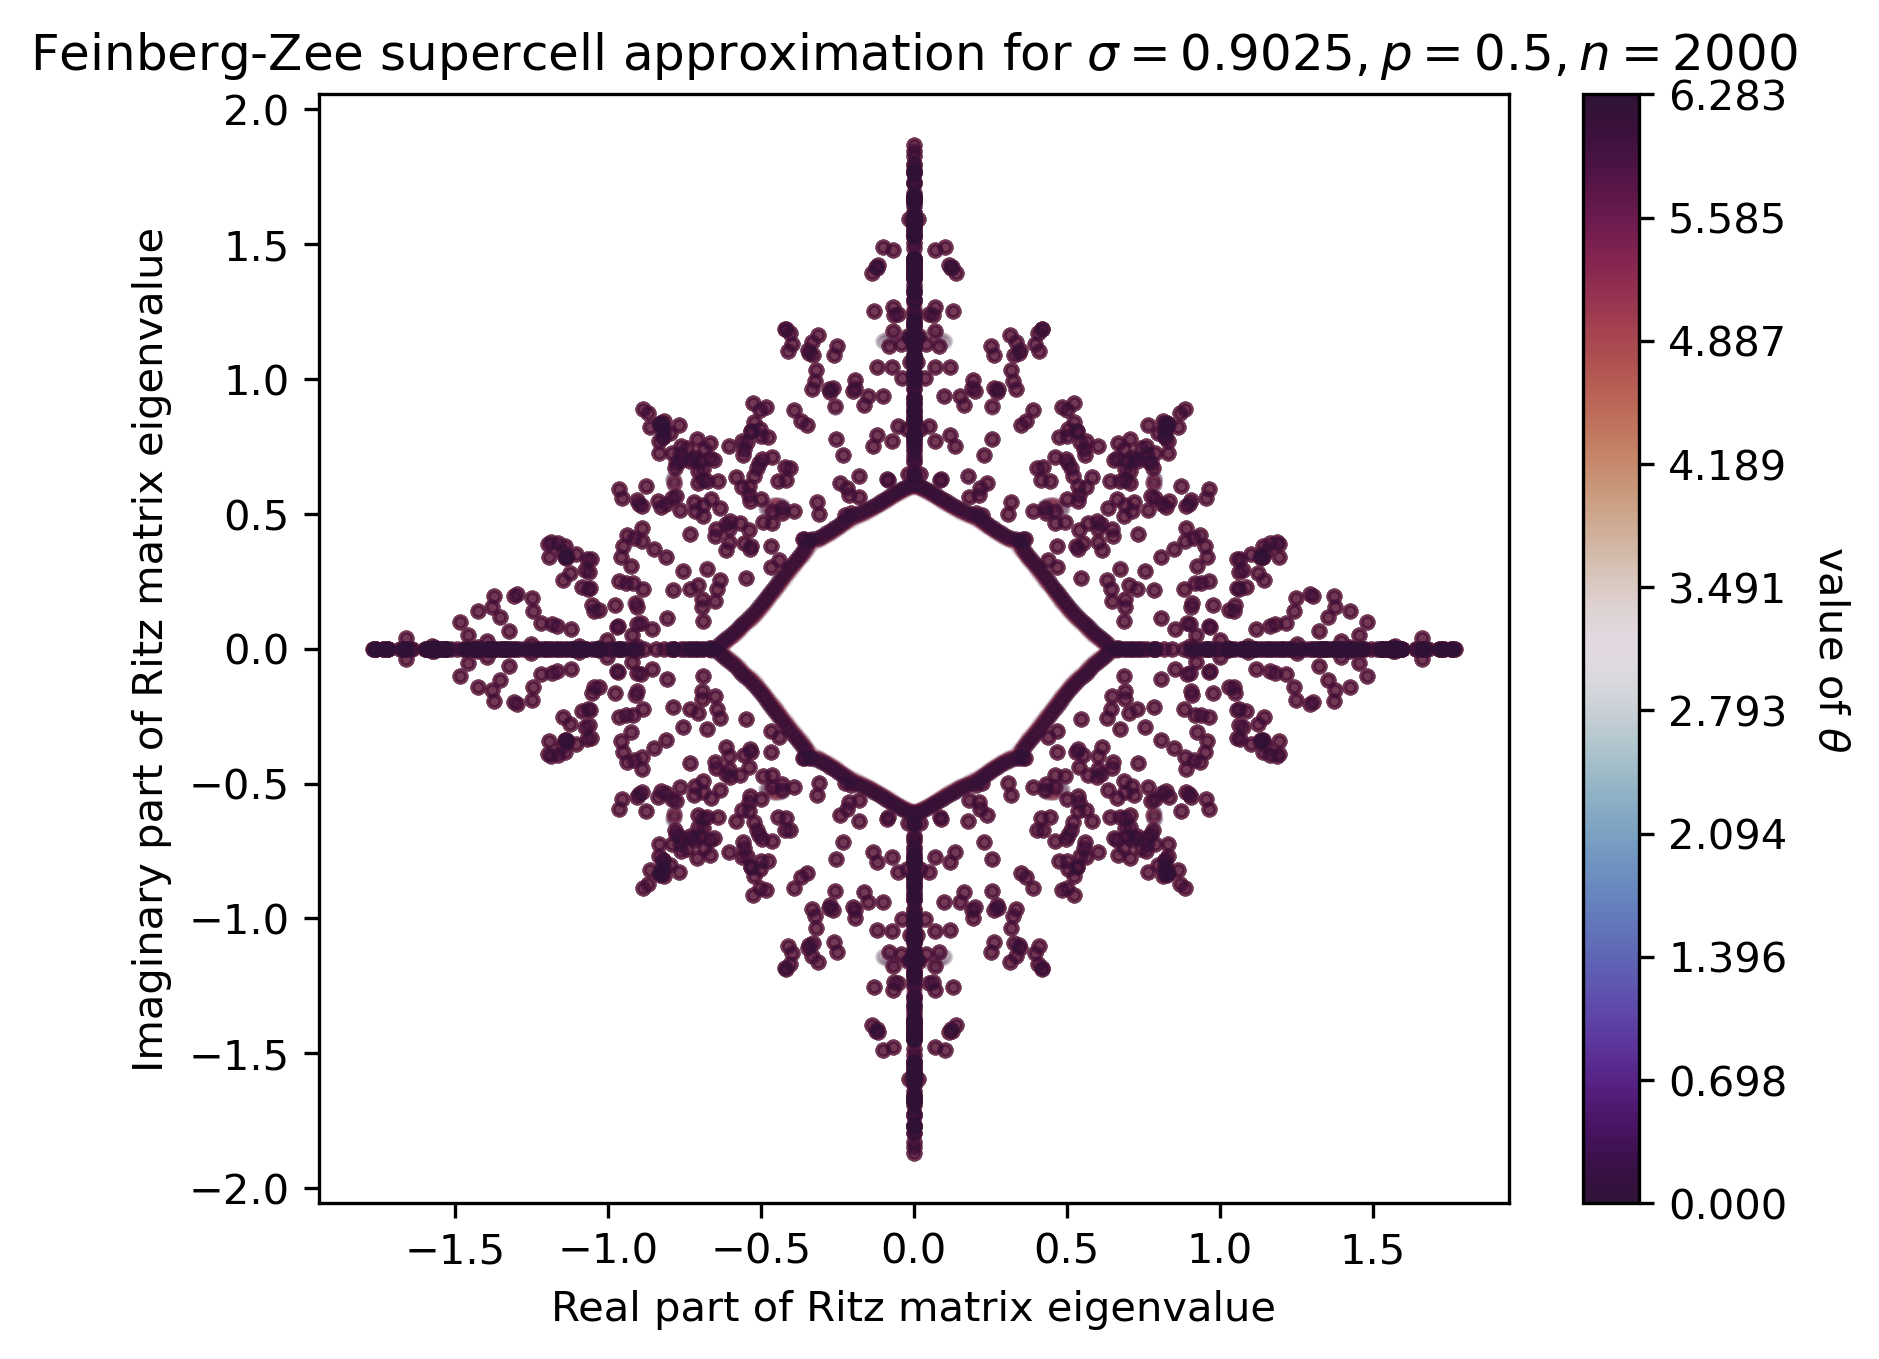
\includegraphics[width=\textwidth]{feinberg-zee-supercell} \end{subfigure}
  \caption{Galerkin and supercell approximations for the Feinberg-Zee operator,
	with matrix size of 2000. Colour is used on the supercell graph to
	distinguish different values of $\theta$, which were 50 evenly
	distributed values between $0$ and $2 \pi$, and the same random
	sequence was used in both cases. One can see the quite startling
	difference between the two; the hole in the supercell approximation.
	Chandler-Wilde and Davies \cite{chandler-wilde2012spectrum} conjecture
	that this hole is in fact present in the actual spectrum of $A^{per}$,
  suggesting that the Galerkin approximation is quite far from the truth
  in this case.}
\label{fig:feinberg-zee}
\end{figure}
\clearpage

\end{document}

